\section{Discussion}
\label{chap:discussion}
Following the descriptive evaluation of the semi-structured interviews, expert interviews and focus group in \hyperref[chap:evaluation]{section \ref{chap:evaluation}}, \hyperref[sub:evaluation-results]{sub-section \ref{sub:evaluation-results}} will do an interpretation of the results of the evaluation steps. \hyperref[sub:method-discussion]{Sub-section \ref{sub:method-discussion}} will critically revisit the methodology described in \hyperref[chap:methodology]{section \ref{chap:methodology}}. Limitations of both methodology and evaluation techniques, which emerged over the course of this thesis, will be described in \hyperref[sub:limitations]{sub-section \ref{sub:limitations}}.

\subsection{Evaluation Results}
\label{sub:evaluation-results}
According to the respondents of the semi-structured interviews, public deliberation enables citizens to actively influence their environment through self-determined organization. Easy access of information is seen as first step to initiate interest and spark discussions. Means currently used for this are generally unspecialized. Generally, tools are used to inform and educate citizens. Although many respondents mentioned the use of Internet pages, only one interviewee addressed the use of a wiki web application for collaboratively collecting information. Online based participation for engaging citizens beyond informing or collecting arbitrary information was generally not considered by any of the respondents.\\
Benefits of using spatially enhanced dialogs in public deliberation were immediately visible for all participants of the evaluation. The ability to grasp proximities and spatial densities of discussion subjects was among the most useful aspects according to the respondents. Interactivity helped to recognize relationships between spatial features and contributions.\\
User interface functions were received generally well by experts and participants of the focus group. Except for some minor deviations, all functions worked as expected. Reactions of both experts were positive. In their opinion, the developed prototype enables supporting spatially enhanced dialogs. Suggestions like geocoding the text of a contribution and user accessible favorite-lists could further enhance the usefulness of the prototype.\\% \todo{Vielleicht noch mehr expert results}\\
\begin{figure}[!h]
    \centering
    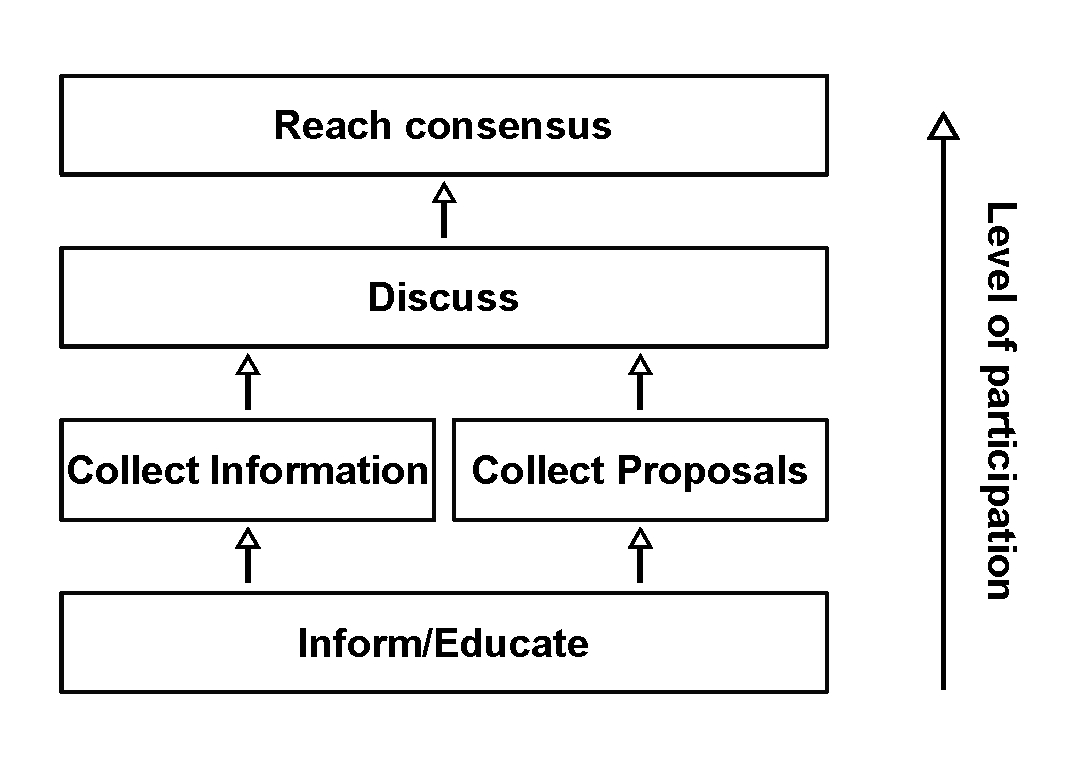
\includegraphics[width=1\columnwidth]{images/my_ladder}
    \caption{Levels of participation. \textit{DialogMap} supports levels up to ``Discuss''. Envisioned use of respondents lies between ``Collect Information'' and ``Collect Proposals''. Levels adapted from Arnstein and colleagues.}
    \label{fig:my_ladder}
\end{figure}
Despite the well reception the concept of spatially referenced discussions, participants of the focus group evaluation showed doubts about broad acceptance of spatial discussion platforms. As respondents of the semi-structured interviews mentioned informing the public as one of the most useful aspects, it becomes apparent that the need for specialized spatial discussion platforms is not seen by evaluation participants. Potential exclusion of groups or persons without Internet access, data privacy, low public acceptance, unclear context and reuse of contributions could be reasons for this reluctance. Despite recognising benefits of spatially enhanced dialogs and understanding the concept, participants suggested to use the developed platform to convey information with spatial aspects. \hyperref[fig:my_ladder]{Figure \ref{fig:my_ladder}} shows the envisioned usage of respondents in correspondence to the theoretical capabilities of \textit{DialogMap}.\\
In retrospect to the research question, public deliberation conducted by citizen initiatives could benefit through the deployment of spatially enhanced dialogs if they feel comfortable to deploy it. Projects like ``Nexthamburg'' and ``Nextkassel'' are good examples for similar systems with broad participation. Further research to determine most important factors for the deployment of spatial discussion platforms in context of public deliberation performed by citizen initiatives has to be conducted.



\subsection{Methodology}
\label{sub:method-discussion}
In order to answer the research question posed in \hyperref[chap:introduction]{section \ref{chap:introduction}}, several steps were taken. A spatial discussion platform prototype was developed to demonstrate the concept of spatially enhanced dialogs, which was then evaluated with overall 13 participants distributed over semi structured interviews, expert interviews and a focus group.\\
In opposition to methods like paper prototyping or interactive mock ups, the development of a full working prototype was chosen. A working prototype, which can be used and tested has several advantages over methods mentioned before. Questions of participants could be answered directly on it. Also, the release of the source code to the public allows future researchers not only to learn from this thesis, but also from the implementation details. The fact that development was performed in an agile manner, with direct feedback of members of a scientific citizen initiative, allowed to further refine the outcome of the development.\\
Qualitative over quantitative evaluation techniques were chosen to explore reasons for acceptance and opinions to the use of spatially enhanced dialogs in a fine grained matter. Also, interviews allow to dynamically react to the respondent to further explore aspects previously not considered by evaluation design. As P7 noted, public participation and deliberation already is highly socially selective. Remarks like this could not have been come up with quantitative evaluation techniques like usability questionnaires.\\

\subsection{Limitations}
\label{sub:limitations}
The development of the prototype was conducted with input of only one scientific citizen initiative. Their influence resulted in a software which serves first and foremost their needs specialized to the sustainability project. For example the multiple categories for the contributions were confusing for people unfamiliar with the background of the sustainability project. Although introduction texts to concept and functionalities as well as videos are included, a real tutorial was not implemented due to limited time available and focus on other last-minute additions, like the ability to upload pictures.\\
Feature-wise, discussions are supported. Users are able to create spatial references and hyperlinks and relate to other spatial references. Discussion contributions are organized linearly and users can express support by favoring contributions. The prototype does not feature functions found in traditional forum softwares like voting, merging of threads, drafting contributions, private messaging to other users or direct moderation. It is also not possible to upload geo data.\\%\todo{Auf suggestions eingehen}\\
The evaluation conducted in this thesis focuses on benefits and support of public deliberation conducted by citizen initiatives. Despite considering user friendliness during the development of the prototype, user friendliness was directly only tested by Tobias Heide.\\
Participants for both the semi-structured interviews as well as the focus group were recruited over mailing-lists of the scientific citizen initiative. This was done to get insights and opinions from real-world citizen activists. Participants were mainly over 40 in age. A more diverse selection of participants or more interviews and focus groups with more participants over longer periods of time could have lead to other results.\\
Additionally legal implication of running such an online platform have to be explored.

%In his ``Twenty years of progress: GIScience in 2010'', Goodchild devotes a section to ``The role of the citizen'' \cite{goodchild2014twenty}. He states

%Following the famous quote of Garson and Biggs \cite{Garson1992_80Percent} that